\begin{frame}[parent={ie:agenda}, hasnext=false, hasprev=false]
	\frametitle{Produto}

	\begin{center}
		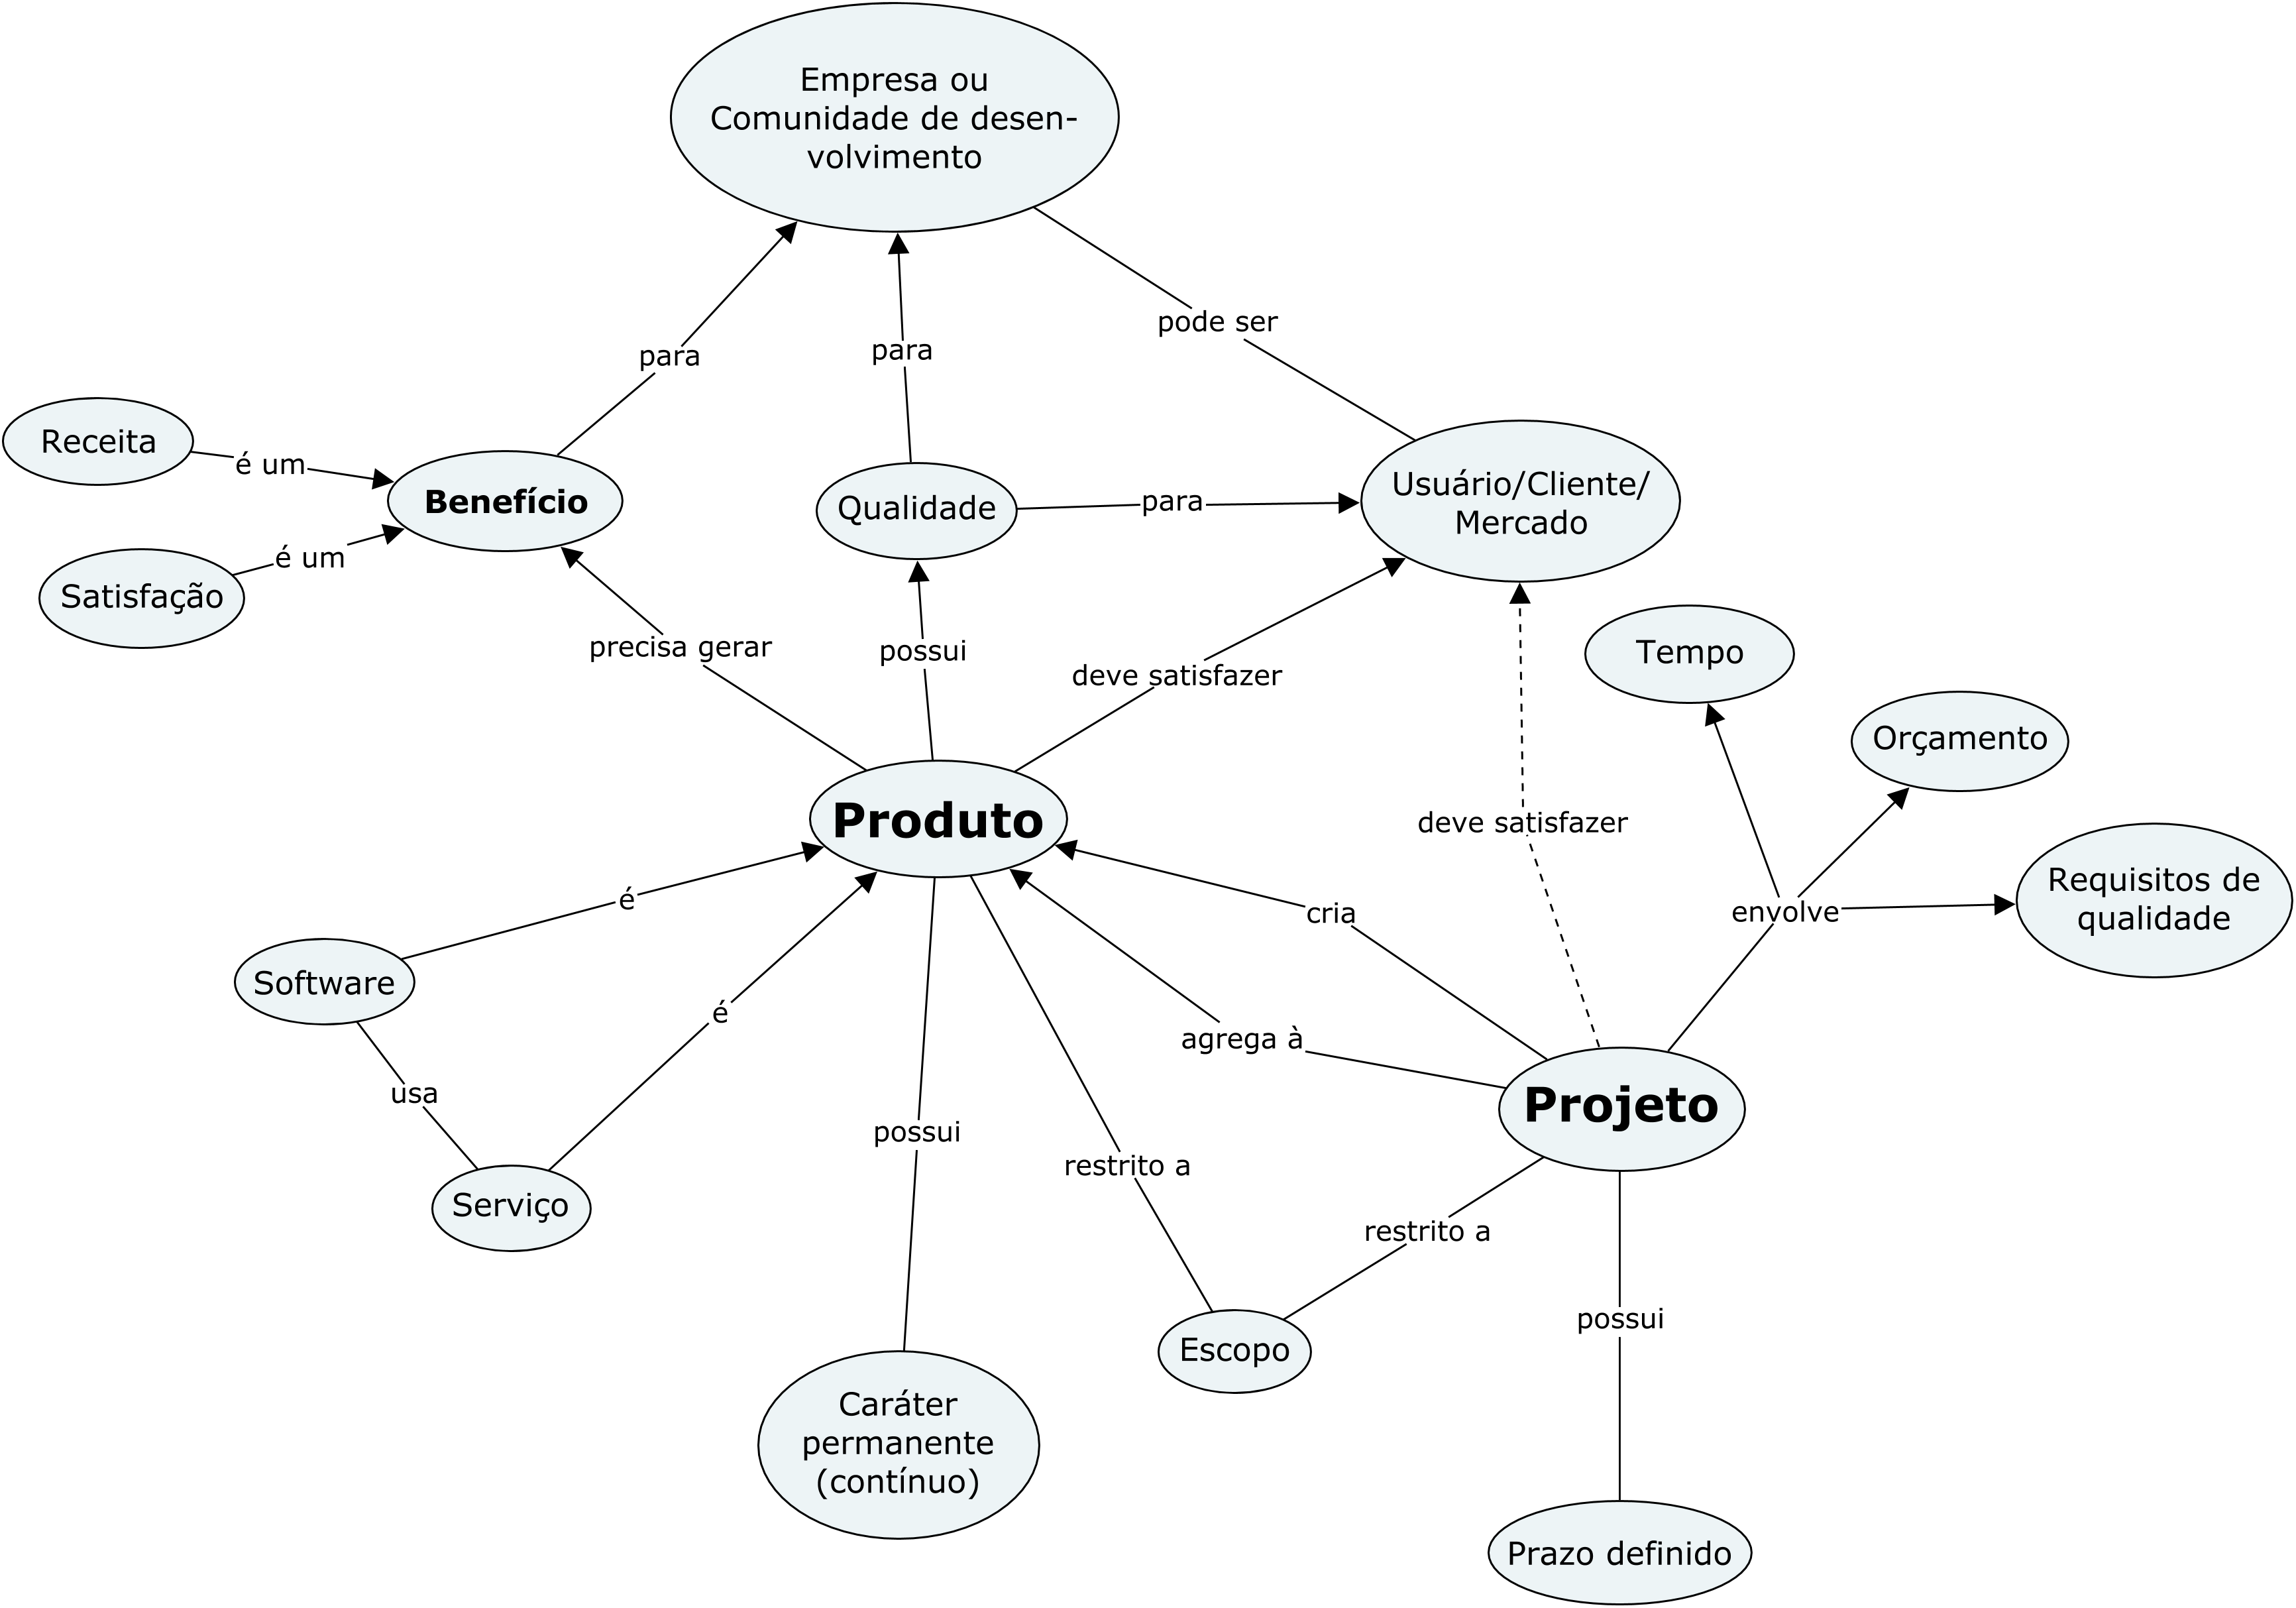
\includegraphics[width=\textwidth]{product}
	\end{center}
\end{frame}


\begin{frame}[parent={ie:agenda}, hasnext=false, hasprev=false]
	\frametitle{Produto}
	
	\begin{block:concept}{Definição}
		Um produto pode ser uma combinação de sistemas, soluções, materiais
		e serviços:
	
		\begin{itemize}
			\item Uma \textbf{solução} é produto específico para cliente
			criado a partir de diferentes produtos, processos e recursos,
			e ajustado para servir os propósitos específicos
			de negócio do cliente.
			
			\item Um \textbf{serviço} é um produto temporário e intangível que é
			resultante da cociração de valor por ao menos uma atividade
			executada entre fornecedor e o cliente e que não implica em
			troca de propriedade.
		\end{itemize}
	\end{block:concept}
		
	\begin{block:fact}{}
		Produtos representam a essência do negócio, como ele prospera,
		cresce e traz lucros para a empresa.
		
		Projetos são o meio para derivar, entregar e suportar produtos
		e outros elementos de negócio relacionados a ele.
	\end{block:fact}
\end{frame}



\begin{frame}
	\frametitle{Produto e Projeto}

	\begin{block:fact}{Sucesso do projeto X Sucesso do produto}
		\begin{itemize}
			\item Sucesso do projeto $\neq$ sucesso do produto
			\item Entretanto, sucesso de projetos é condição para sucesso do produto.
			\item Escopo e qualidade
		\end{itemize}
	\end{block:fact}
	
	\begin{block:ie}{Exemplos}
		Windows (sistema operacional): inicialmente um produto ruim, mas
		sucessivos projetos bem sucedidos tornaram-no em um produto de
		sucesso.
	
		Digg (agregador de notícias): inicialmente um bom produto, mas
		sucessivos projetos mal sucedidos levaram o produto à bancarrota.
	\end{block:ie}
\end{frame}

